\underline{Synchronizacja tożsamościowa} - oba sygnały opisujące dynamikę układów są identyczne.

\underline{Synchronizacja uogólniona} - odpowiadające sobie zmienne są proporcjonalne (np. amplituda)

Aby doszło do powyższych synchronizacji układy muszą być sprzężone.\newline
\newline
\underline{Synchronizacja fazowa} - wprowadza się pojęcie sygnału analitycznego: \newline
$ \psi(t) = s(t) + j\tilde{s}(t) = Ae^{j\omega\phi (t)} $, gdzie:\newline
$ \tilde{s}(t) $ - transformata Hilberta sygnału $ s(t) $,\newline
$ \phi (t) $ - faza sygnału $ s(t) $.

Układy są zsynchronizowane fazowo jeśli różnica faz $ |n\psi_1(t) + m\psi_2(t)| = const. $

Istnieje wiele układów pomiędzy którymi może wystąpić jedynie synchronizacja fazowa. Przykładem są układy impulsowe jak pewien gatunek świetlików żyjący w Indonezji.

\underline{Model Kuramoto} - model opisujący synchronizację w grupie sprzężonych oscylatorów.

Opisuję układ $ N $ rotatorów. Tempo zmiany fazy $ \theta_i $, $ i $-tego rotatora:\newline
$ \dfrac{\theta_i}{dt} = \omega_{0}^i + \dfrac{k}{N} \sum_{j=1}^N \sin (\theta_i - \theta_j) $, gdzie:\newline
$ \omega_{0}^i $ - naturalna częstość rotatora $ i $,\newline
$ k $ - amplituda sprzężenia.


Gdy $ k > 0 $ fazy rotatorów powinny się zsynchronizować:
\begin{itemize}
	\item Jeśli rotator $ i $ spóźnia się względem średniego rotatora $ \tilde{\theta}(t) - \theta_i(t) > 0 $, wtedy rotator $ i $ przyśpiesza.
	\item Gdy rotator $ i $ śpieszy się względem średniego rotatora $ \tilde{\theta}(t) - \theta_i(t) < 0 $, wtedy rotator $ i $ zwalnia.
\end{itemize}

Istnieje pewna wartość krytyczna amplitudy sprzężenia $ k_C $, powyżej której scyntylatory się zsynchronizują.  Dla $ N = 2 $ wartość ta jest zależy od różnicy naturalnych częstości rotatorów $ |\omega^0_1 - \omega^0_2| $. Dla $ N \gg 1 $, gdy naturalne częstości pochodzą z rozkładu $ \mathcal{N}(0, \sigma^2) $ wtedy wartość krytyczna zależy od $ \sigma $. \textbf{Wniosek}: Im większe zróżnicowanie naturalnych częstości rotatorów tym trudniej zsynchronizować układ.

\underline{Synchronizacja grupy świetlików}

Układ składa się z $ N $ oscylatorów.

Naładowanie oscylatora definiuje się następująco:\newline

$ U(\phi(t)) = C(1 - e^{-\gamma \phi(t)}) $, gdzie:\newline
$ \phi(t) $ - faza oscylatora.

Gdy $ U(\phi) = 1 $, następuje rozładowanie oscylatora ($ U(\phi) = 0 $) i każdy ze sprzężonych oscylatorów ładuje się o $ \epsilon $ co jednocześnie "przesuwa" fazy tych oscylatorów.

Kształt funkcji naładowania powoduje, że po pewnym czasie dochodzi do sprzężenia faz oscylatorów. 
\begin{figure} [H]
	\centering
	\begin{subfigure}{.55\textwidth}
		\centering
		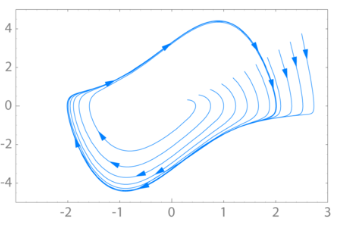
\includegraphics[width=1.0\linewidth]{EDMIIssues/Figures/pol.png}
	\end{subfigure}
	\caption{"Wpadanie" w cykl graniczny oscylatora Pola dla różnych warunków początkowych.}
	\label{pol}
\end{figure}
\underline{W oscylatorach nieliniowych z cyklem granicznym} faza, amplituda oraz częstość są własnościami stanu oscylatora. Po pewnym stanie nieustalonym układ osiąga cykl graniczny (rys~\ref{pol}), niezależnie od warunków początkowych. Przykładem takiego oscylatora jest oscylator van der Pola opisany równaniem:\newline

$ \dfrac{d^2 x}{dt^2} + \mu (x^2 - 1)\dfrac{dx}{dt} + x = 0 $

Sprzężone oscylatory nieliniowe zazwyczaj starają się "śpiewać wspólnie" tzn. z jedną częstością przy czym zazwyczaj częstość "silniejszego" (np. tego o większej amplitudzie) bierze górę, lub znajdują wspólną częstość - zazwyczaj ustalony stosunek ich częstości własnych. Zjawisko sprzężenia częstości (drgania synfazowe) jest rodzajem synchronizacji. Oscylatory liniowe tego nie potrafią: nie są w stanie zmieniać swej częstości. Nawet sprzężone, nieliniowe oscylatory nie zawsze sobie radzą ze znalezieniem wspólnej częstości, stąd wynika \underline{kwaziperiodyczność} (ruch z kilkoma niewspółmiernymi częstościami)  lub \underline{ruch chaotyczne} (trajektoria układu w przestrzeni fazowej jest otwarta, ale ograniczona przestrzennie).

Dzięki swoim własnością oscylatory nieliniowe są dobrymi kandydatami do:
\begin{itemize}
	\item Modelowania zjawisk biologicznych - wiele rytmów jest cechą własną gatunku, niezależną od warunków początkowych oraz względnie małych zmian otoczenia, a jednocześnie muszą być w zgodzie z rytmami natury (np. dzień/noc)
	\item do zastosowań technicznych w telekomunikacji, czy w technikach pomiarowych.
\end{itemize}

Synchronizacja fazowa znalazła zastosowanie m.in. w medycynie, gdzie pozwala analizować oddziaływanie oddechu z rytmem serca.
